\section{Vision Simultaneous Localization and Mapping (VSLAM)}
\label{sec:vslam}

Pepper needs a model (a map) of the environment to support other tasks, mainly auto-navigation, but a prior map is often not available in various home scenarios, so SLAM find its application. 
The stereo camera data is mainly used by a visual SLAM module, together with laser (very limited) and odom (has significant error) data. 
Our VSLAM algorithm is based on RTAB-Map, a graph-optimized based VSLAM algorithm, and have been modified for Pepper's sensors. 
Odom and laser scan data make the initial pose estimation, then stereo data serves for appearance-based loop closure detection to optimize local and global pose. 
VSLAM can get a 3D point cloud, we make a projection to get a 2D grid map for navigation. 
Having map and Pepper’s size parameters, we use DWA (Dynamic Window Apporach) to plan the path and fuse vision, laser and sonar data to make real-time obstacle avoidance (mainly for dynamic scene), a series of motion command will be sent to NAOqi APIs, so Pepper can navigate to its goal points itself.

\begin{figure}[h]
    %\centerline{    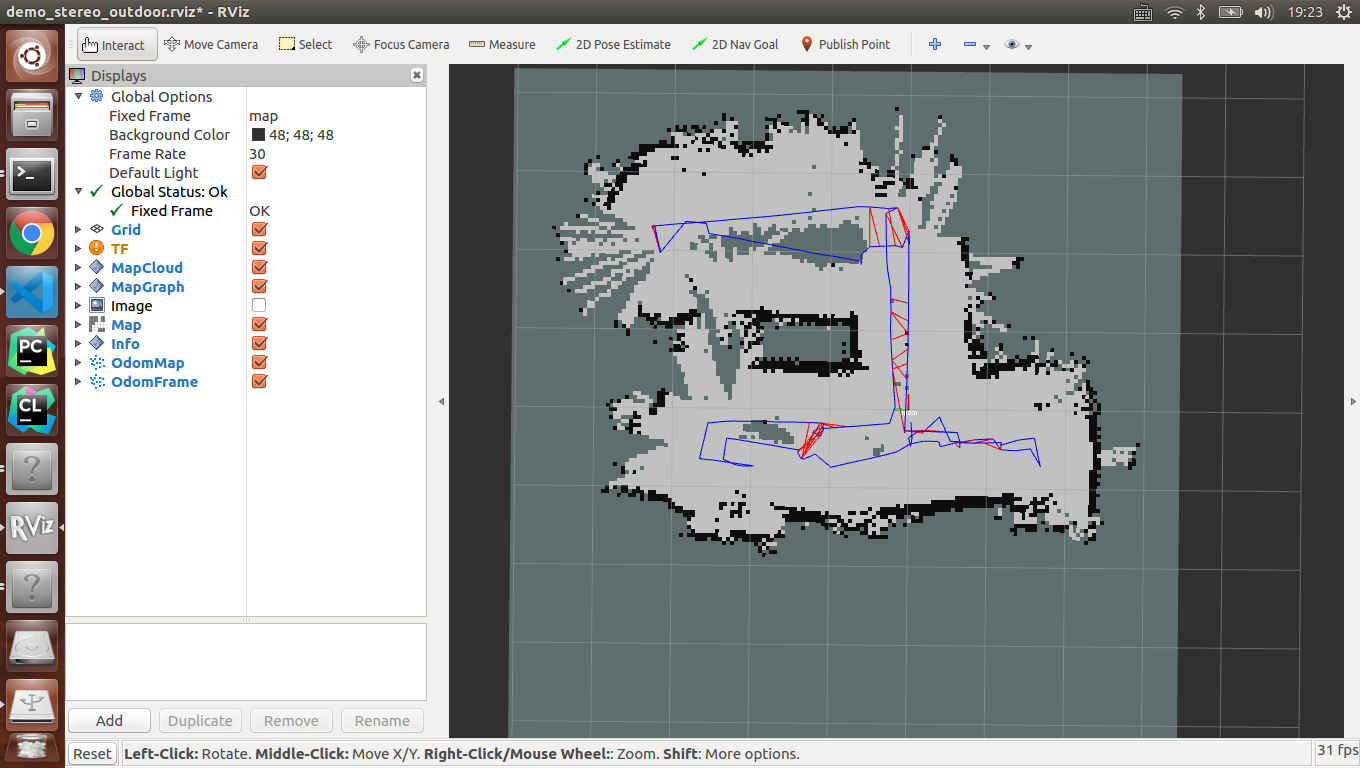
\includegraphics[width=1.\textwidth]{figs/vslam_shortcut.png} }  
    \centering
    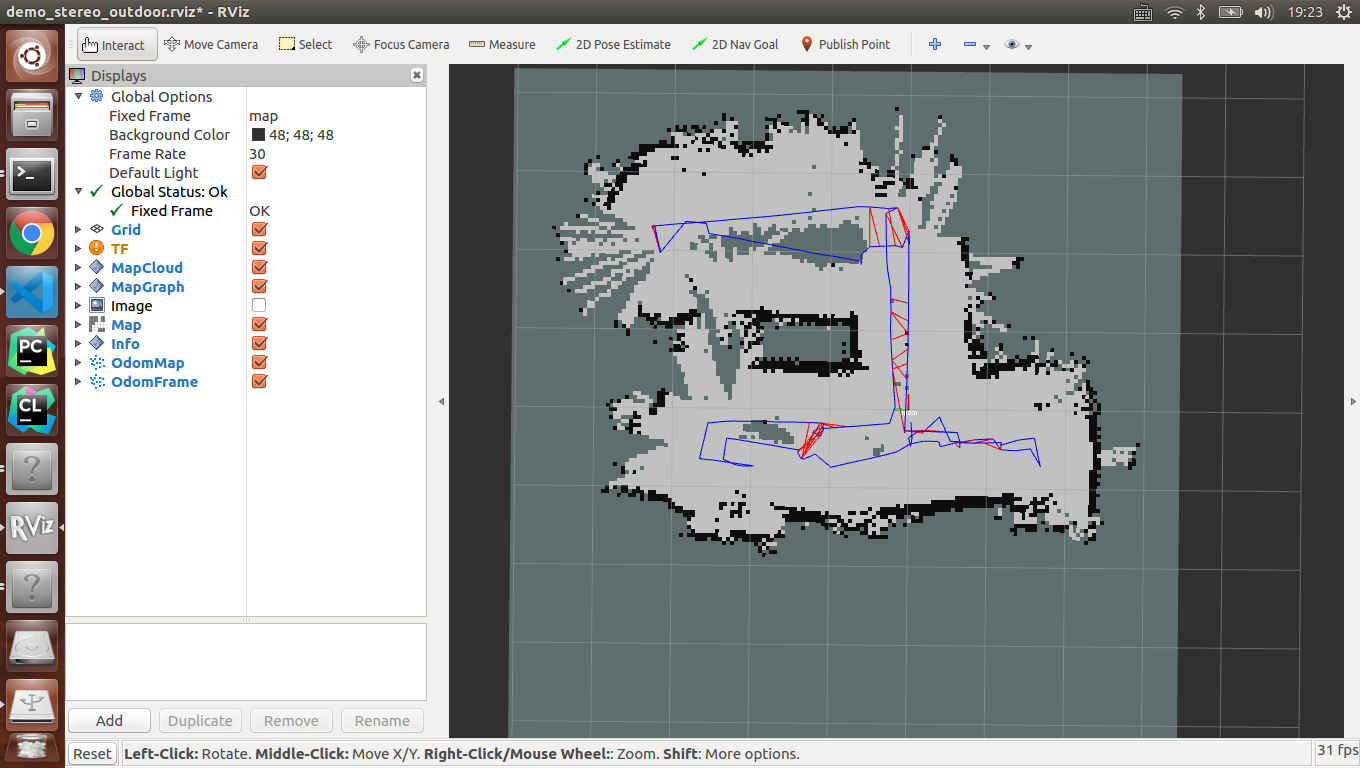
\includegraphics[width=1.\textwidth]{figs/vslam_shortcut.png}
    \caption{SLAM and navigation on ROS}
    \label{fig:vslam}
\end{figure}